\section{Durchführung}

\subsection{Aufbau}
Eine schematische Darstellung der Messappatur ist in Abbildung \ref{fig:aufbau} zu sehen.
%Es sei angemerkt, dass der hier verwendete Laser unpolarisiertes monochromatisches Licht entsendet.
Sie besteht im Wesentlichen aus einem Laser, der monochromatisches Licht erzeugt 
(hier unterscheidet sich der Aufbau etwas von der Darstellung in der Abbildung).
Da dieses zunächst unpolarisiert ist, können zwei verstellbare Polarisatoren auf der Schiene aufgebaut werden, um linear polaristeres 
Licht zu erzeugen.
Der erste Polarisator ist dabei stets auf \qty{45}{\degree} gestellt.
Der zweite Polarisator wird für parallele Polarisation auf \qty{90}{\degree} (parallel zur Zeichenebene in Abbildung \ref{fig:aufbau})
und für senkrechte Polarisation auf \qty{0}{\degree} (aus der Zeichenebene heraus) gestellt.
Das Licht trifft auf einen Silizium-Spiegel, der sich auf einem Drehteller mit Winkelskala befindet, sodass der Einfallswinkel
am Spiegel variiert und abgelesen werden kann.
Außerdem gibt es ein schwenkbares Photoelement, dessen Strom proportional zur Intensität des Lichtes ist.
Durch den beweglichen Arm kann das Element in den Reflexionsstrahl schwenken.

\begin{figure}[H]
    \centering
    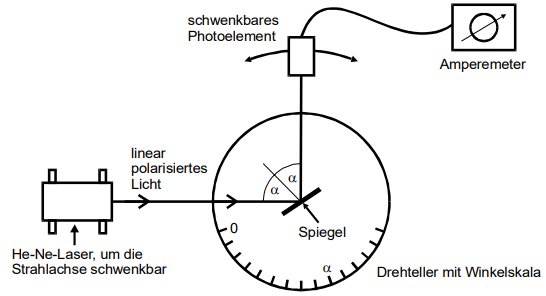
\includegraphics[height = 5.5 cm]{Abbildungen/aufbau.png}
    \caption{Schematische Darstellung des Versuchsaufbaus \cite{man:v407}.}
    \label{fig:aufbau}
\end{figure}


\subsection{Vorbereitung der Messung}
Im ersten Schritt wird der Probenhalter (vgl. Abblidung \ref{fig:goniometer}) vom Goniometer gelöst, um den Strahlengang frei zu machen.
Der Drehteller wird genullt.
Anschließend werden die beiden Polarisatoren auf der Schiene fixiert und wie oben beschrieben eingestellt.
Hierbei werden die Intensitäten für das parallel und senkrecht polarisierte Licht bei einem Einfallswinkel von \qty{0}{\degree} notiert.
Die beiden Werte sollten in etwa gleich groß sein.
Im nächsten Schritt wird der Probenhalter wieder auf das Goniometer geschraubt und der Spiegel in Höhe und Neigung entsprechend eingestellt.
Der reflektierte Laserstrahl sollte dabei die gleiche Höhe wie der einfallende Lichtstrahl haben.
Bei einem Einfallswinkel von \qty{0}{\degree} sollte der reflektierte Strahl dann wieder auf die Öffnung des Lasers treffen.

\begin{figure}[H]
    \centering
    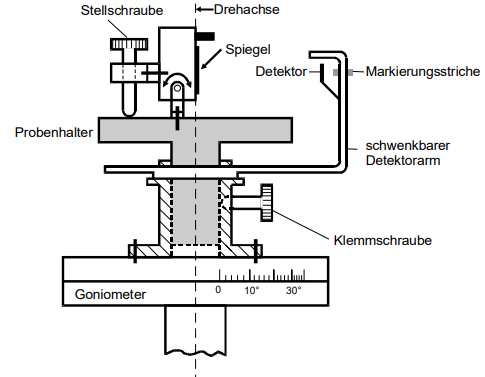
\includegraphics[height = 6 cm]{Abbildungen/goniometer.png}
    \caption{Schematische Darstellung des Goniometers inklusive Probenhalter \cite{man:v407}.}
    \label{fig:goniometer}
\end{figure}


\subsection{Messprogramm}
Der Einfallswinkel wird in einem Intervall von \qtyrange{5}{88}{\degree} in Schritten von \qty{5}{\degree} erhöht.
In der Nähe des Brewsterwinkels (zwischen \qtyrange{75}{80}{\degree}) wird dabei mit \qty{1}{\degree} Schritten genauer gemessen, 
um den Brewsterwinkel bestimmen zu können.
Bei jedem eingestellten Winkel wird der zweite Polarisator jeweils für senkrecht und parallel polaristeres Licht eingestellt
und die Stromstärke notiert.
Ferner wird der Detektor ein wenig zur Seite bewegt, um die Nullintensität für jeden Winkel messen zu können 
und systematische Fehler zu minimieren.

